\documentclass[otchet]{SCWorks}
% Тип обучения (одно из значений):
%    bachelor   - бакалавриат (по умолчанию)
%    spec       - специальность
%    master     - магистратура
% Форма обучения (одно из значений):
%    och        - очное (по умолчанию)
%    zaoch      - заочное
% Тип работы (одно из значений):
%    coursework - курсовая работа (по умолчанию)
%    referat    - реферат
%  * otchet     - универсальный отчет
%  * nirjournal - журнал НИР
%  * digital    - итоговая работа для цифровой кафдры
%    diploma    - дипломная работа
%    pract      - отчет о научно-исследовательской работе
%    autoref    - автореферат выпускной работы
%    assignment - задание на выпускную квалификационную работу
%    review     - отзыв руководителя
%    critique   - рецензия на выпускную работу
% Включение шрифта
%    times      - включение шрифта Times New Roman (если установлен)
%                 по умолчанию выключен

\usepackage{preamble}
\captionsetup[figure]{font= normalsize, labelfont=normalsize}
\renewcommand\theFancyVerbLine{\small\arabic{FancyVerbLine}}

\begin{document}

% Кафедра (в родительном падеже)
\chair{информатики и программирования}

% Тема работы
\title{DevOps: его роль в современной разработке программного обеспечения}

% Курс
\course{3}

% Группа
\group{351}

% Факультет (в родительном падеже) (по умолчанию "факультета КНиИТ")
% \department{факультета КНиИТ}

% Специальность/направление код - наименование
% \napravlenie{02.03.02 "--- Фундаментальная информатика и информационные технологии}
% \napravlenie{02.03.01 "--- Математическое обеспечение и администрирование информационных систем}
% \napravlenie{09.03.01 "--- Информатика и вычислительная техника}
\napravlenie{09.03.04 "--- Программная инженерия}
% \napravlenie{10.05.01 "--- Компьютерная безопасность}

% Для студентки. Для работы студента следующая команда не нужна.
% \studenttitle{Студентки}

% Фамилия, имя, отчество в родительном падеже
\author{Устюшина Богдана Антоновича}

% Заведующий кафедрой 
\chtitle{доцент, к.\,ф.-м.\,н.}
\chname{С.\,В.\,Миронов}

% Руководитель ДПП ПП для цифровой кафедры (перекрывает заведующего кафедры)
% \chpretitle{
%     заведующий кафедрой математических основ информатики и олимпиадного\\
%     программирования на базе МАОУ <<Ф"=Т лицей №1>>
% }
% \chtitle{г. Саратов, к.\,ф.-м.\,н., доцент}
% \chname{Кондратова\, Ю.\,Н.}

% Научный руководитель (для реферата преподаватель проверяющий работу)
\satitle{доцент, к.\,п.\,н.} %должность, степень, звание
\saname{М.\,С.\,Портенко}

% Руководитель практики от организации (руководитель для цифровой кафедры)
\patitle{доцент, к.\,ф.-м.\,н.}
\paname{С.\,В.\,Миронов}

% Руководитель НИР
\nirtitle{доцент, к.\,п.\,н.} % степень, звание
\nirname{В.\,А.\,Векслер}

% Семестр (только для практики, для остальных типов работ не используется)
\term{5}

% Наименование практики (только для практики, для остальных типов работ не
% используется)
\practtype{учебная}

% Продолжительность практики (количество недель) (только для практики, для
% остальных типов работ не используется)
\duration{2}

% Даты начала и окончания практики (только для практики, для остальных типов
% работ не используется)
\practStart{01.07.2022}
\practFinish{13.01.2023}

% Год выполнения отчета
\date{2023}

\maketitle

% Включение нумерации рисунков, формул и таблиц по разделам (по умолчанию -
% нумерация сквозная) (допускается оба вида нумерации)
% \secNumbering

\tableofcontents

% Раздел "Обозначения и сокращения". Может отсутствовать в работе
% \abbreviations
% \begin{description}
%     \item ... "--- ...
%     \item ... "--- ...
% \end{description}

% Раздел "Определения". Может отсутствовать в работе
% \definitions

% Раздел "Определения, обозначения и сокращения". Может отсутствовать в работе.
% Если присутствует, то заменяет собой разделы "Обозначения и сокращения" и
% "Определения"
% \defabbr

\intro

Отчёт по теории графов. \textbf{Используемый язык} -- C++.

Каждая функция в файле \texttt{Tasks.cpp} (приложение \ref{Tasks}) выполняет одно из заданий. Они используют алгоритмы, описанные в файле \texttt{Algos.cpp} (приложение \ref{Algos}).

В файле \texttt{Graph.cpp} (приложение \ref{Graph}) представлена реализация графа, не пересекающаяся с консольным описанием интерфейса. Описание консольного интерфейса описано в файле \texttt{App.cpp} (приложение \ref {App}).

Все файлы взаимодействуют друг с другом посредством подключения .h (хедеров) соответствующих файлов.

Функции интерфейса используются в функции \texttt{main} (приложение \ref{Main}) в главном файле \texttt{main.cpp}.

В отчёте прилагаются изображение графа и скриншоты результата работы программы с файлами из приложения \ref{Json-файлы}, в которых хранятся графы.

\section{Задание 1: Cоздание класса графов}

В первом задании предлагалось создать свой собственный класс графов, в который входят:

\begin{enumerate}
\item Структуру хранения графа (список смежности или список рёбер)
\item Конструкторы (пустой граф, граф из файла, конструктор-копию)
\item Методы (добавления/удаления вершин, добавления/удаления рёбер или дуг, вывод списка смежности в файл, т.е. сохранения графа)
\item Должны поддерживаться как ориентированные/неориентированные графы
\item Должен быть создан минималистичный консольный интерфейс
\end{enumerate}

Структура хранения выбрана как словарь словарей (\texttt{map<map<string, int>\.>}): то есть у каждой вершины есть \texttt{map}, который соответствует вершинам, с которыми она смежна (в случае неориентированного графа) или вершинам, в которые идут дуги (в случае ориентированного графа). 

Представлены конструкторы на основе:
\begin{enumerate}
\item Bool-переменной \texttt{isOriented}, которая определяет, является ли граф ориентированным или нет (поддержка различия двух графов);
\item Файла, в котором граф представляется в json-формате с помощью библиотеки \textit{nlohmann-json};
\item Ссылки на константное значение класса графа -- конструктор копирования.
\end{enumerate}

\textbf{Написать примеры создания графа}

В нём созданы:
\begin{enumerate}
\item \texttt{enum string\_code} -- введённая пользователем строка на основе функции Hashing будет преобразовываться в номер для выполнения определённой команды.
\item \texttt{CommandMessage()} -- выводит справку о поддерживаемых командах, появляется при старте программы и вызове функции \texttt{help} (h)
\item \texttt{CreateGraph} -- интерфейс создания графа (вызывается при пустом файле, указанном в переменной \texttt{DATA\_FILE\_1} имени графа, используемой в главном файле \texttt{main.cpp}).
\item Функция \texttt{PrintVertices} -- выводит все вершины графа в виде списка в консоли.
\item Функция \texttt{AddVertice} -- добавляет вершину к текущему графу, в котором запущена программа.
\item Функция \texttt{RemoveVertice} -- удаляет вершину из текущего графа.
\item Функция \texttt{AddEdge} -- добавляет ребро/дугу к текущему графу.
\item Функция \texttt{RemoveEdge} -- удаляет ребро/дугу у текущего графа.
\item Функция \texttt{ChangeWeight} -- изменяет вес ребра в текущем графе.
\item Функция \texttt{Unweight} -- изменяет вес всех рёбер на 1.
\end{enumerate}

Все исключительные ситуации (ребра при изменении веса или удалении не существует, не существует одной из вершин при добавлении ребра, добавление уже существующей вершины и прочие) обрабатываются внутри класса ещё на этапе выполнения метода классом графа. Методы интерфейса App просто вызывают для переданного им параметра (графа) методы, реализованные внутри класса графа, что позволяет перенести всю логику обработки некорректных ситуаций в класс графа.

Также дополнительно в \texttt{App.cpp} существует функция \texttt{is\_number}, проверяющий корректность введённого числа при вводе веса рёбер (они могут быть лишь целыми числами, положительными, отрицательным или нулём).

\begin{figure}[H]
	\center{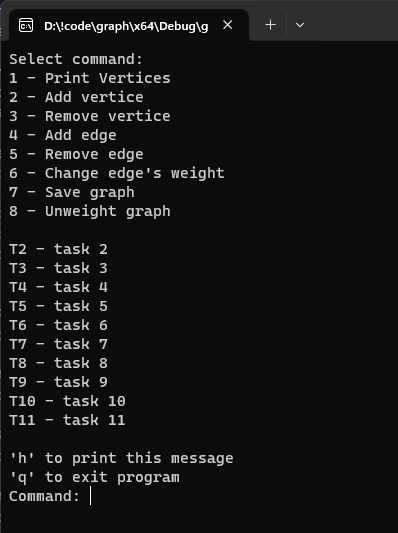
\includegraphics[scale=0.8]{pics/task1_1}}
	\caption{Стартовое сообщение}
	\label{pic1_1}
\end{figure}

\begin{figure}[H]
	\center{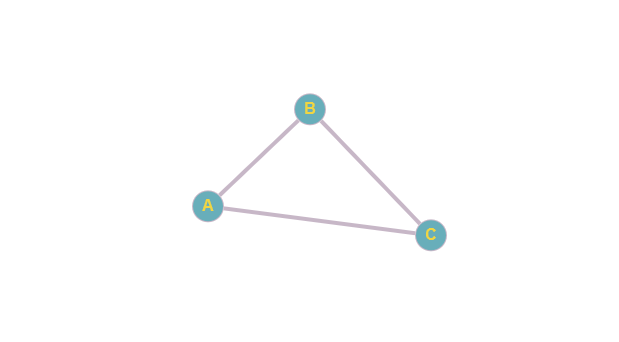
\includegraphics[scale=0.7]{pics/gr1_1}}
	\caption{Граф 1}
	\label{gr1_1}
\end{figure}

\begin{figure}[H]
	\center{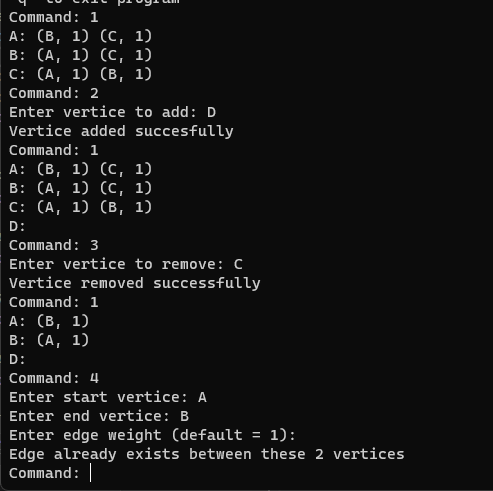
\includegraphics[scale=0.7]{pics/task1_2}}
	\caption{Пример использования функций 1}
	\label{pic1_2}
\end{figure}

\begin{figure}[H]
	\center{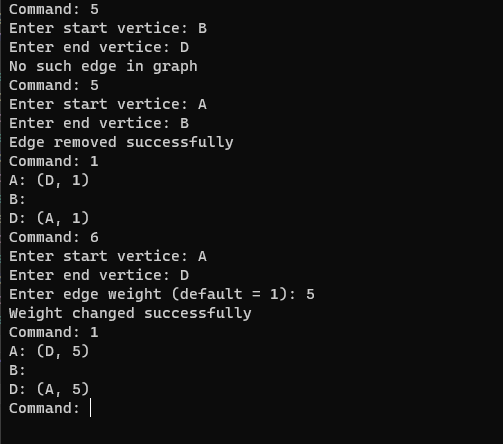
\includegraphics[scale=0.7]{pics/task1_3}}
	\caption{Пример использования функций 2}
	\label{pic1_3}
\end{figure}

\section{Задание 2: Список смежности Ia}

\textbf{Задание: Вывести все вершины орграфа, смежные с данной.}

Обычный перебор используемого map для получения всех соседних вершин. Здесь понятие смежности я отождествляю с существованием дуги.

\begin{figure}[H]
	\center{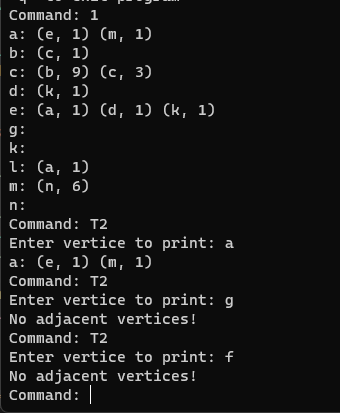
\includegraphics[scale=1]{pics/task2_1}}
	\caption{Задание 2}
	\label{pic2_1}
\end{figure}

\begin{figure}[H]
	\center{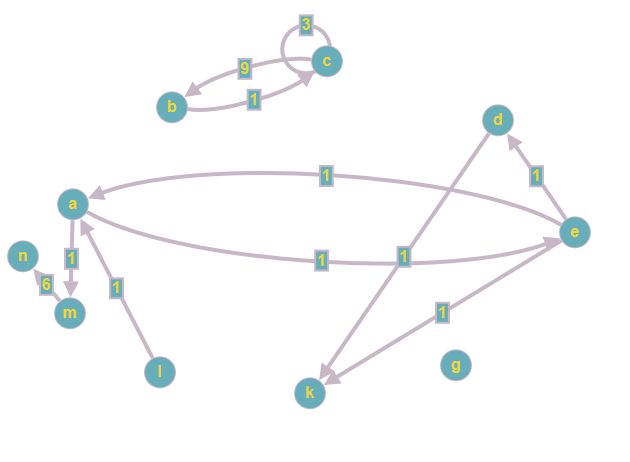
\includegraphics[scale=0.7]{pics/gr2_1}}
	\caption{Граф 2}
	\label{gr2_1}
\end{figure}

\section{Задание 3: Список смежности Ia}

\textbf{Задание: Вывести те вершины, полустепень исхода которых больше, чем у заданной вершины.}

Сначала вводим заданную вершину, затем проходим по списку смежности (первый map) и смотрим количество элементов в каждом внутреннем map. Если их количество больше, то выводим вершину. При несуществующей вершине выводятся все вершины, т.е. изолированные вершины и вершины, отсутствующие в графе, по полустепени захода отождествляются.

\begin{figure}[H]
	\center{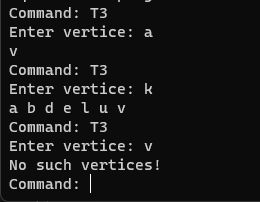
\includegraphics[scale=1]{pics/task3_1}}
	\caption{Задание 3}
	\label{pic3_1}
\end{figure}

\begin{figure}[H]
	\center{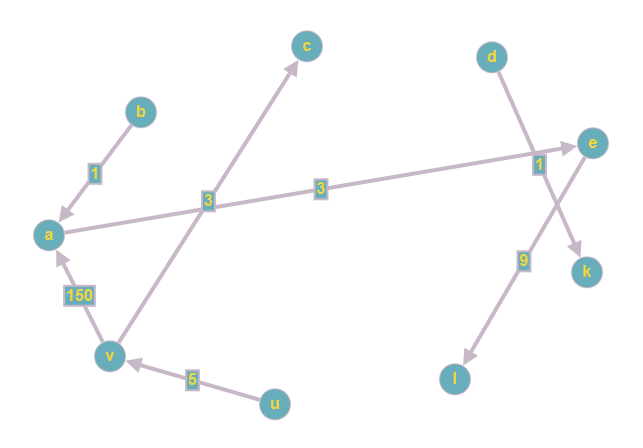
\includegraphics[scale=0.7]{pics/gr3_1}}
	\caption{Граф 3}
	\label{gr3_1}
\end{figure}

\section{Задание 4: Список смежности Ib: несколько графов}

\textbf{Задание: Построить орграф, являющийся симметрической разностью по дугам двух заданных орграфов (множество вершин получается объединением вершин исходных орграфов).}

Если один граф неориентированный, а второй ориентированный (или наоборот), то алгоритм говорит, что графы несовместны.

Алгоритм просматривает списки смежности двух графов, добавляет в новый граф все вершины, которые он встретил (не более одного раза). Далее перебираем всевозможные пары вершин нового графа: если такая пара встретилась лишь в одном списке смежности исходных двух графов (либо в первом, либо во втором), то добавляем эту пару (ребро) в новый граф, иначе игнорируем. В конце формируем граф на основе нового списка смежности.

\begin{figure}[H]
	\center{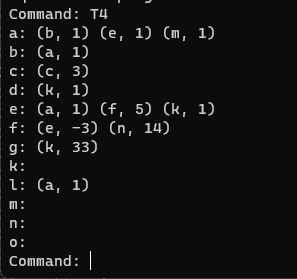
\includegraphics[scale=1.2]{pics/task4_1}}
	\caption{Задание 4}
	\label{pic4_1}
\end{figure}

\begin{figure}[H]
	\center{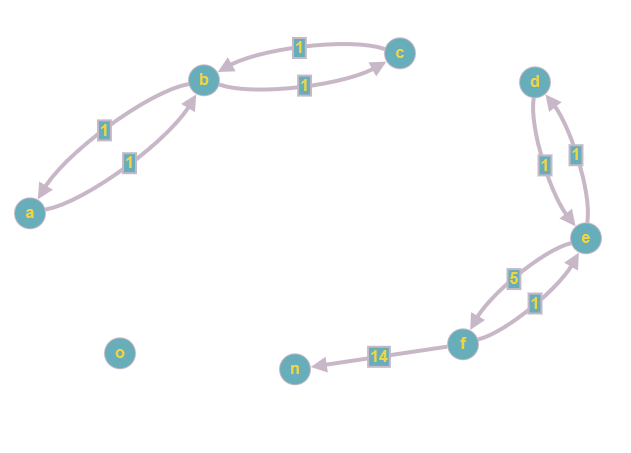
\includegraphics[scale=0.7]{pics/gr4_1}}
	\caption{Граф 4.1}
	\label{gr4_1}
\end{figure}

\begin{figure}[H]
	\center{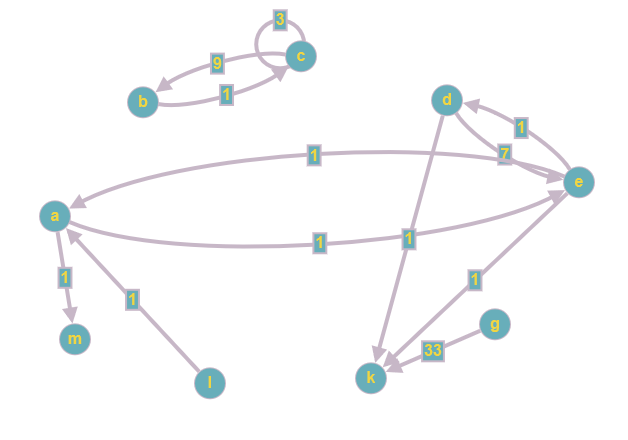
\includegraphics[scale=0.7]{pics/gr4_2}}
	\caption{Граф 4.2}
	\label{gr4_2}
\end{figure}

\begin{figure}[H]
	\center{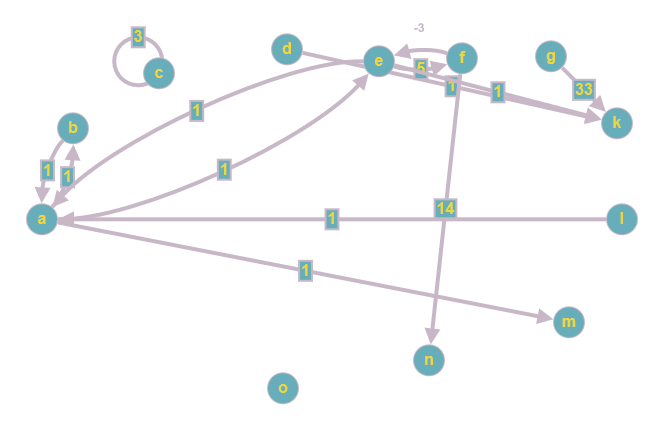
\includegraphics[scale=0.7]{pics/gr4_res}}
	\caption{Граф симметричной разности}
	\label{gr4_res}
\end{figure}

\section{Задание 5: Обходы графа II}

\textbf{Задание: Найти все вершины орграфа, недостижимые из данной.}

Обычное использование BFS: выводим вершины, которые после прохода BFS остались непомеченными. Если все вершины достижимы, выводим об этом сообщение.

\begin{figure}[H]
	\center{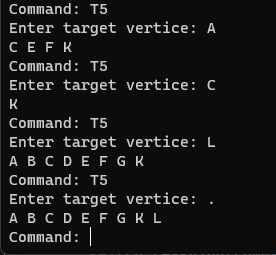
\includegraphics[scale=1.2]{pics/task5_1}}
	\caption{Задание 5}
	\label{pic5_1}
\end{figure}

\begin{figure}[H]
	\center{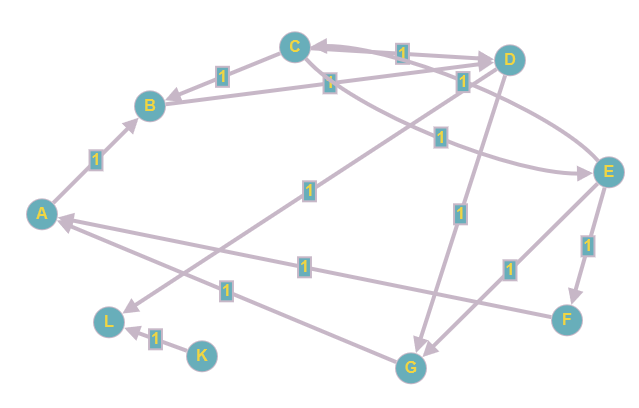
\includegraphics[scale=0.7]{pics/gr5_1}}
	\caption{Граф 5}
	\label{gr5_1}
\end{figure}

\section{Задание 6: Обходы графа II}

\textbf{Задание: Вывести все пути из u в v.}

Используем модифицированный алгоритм DFS: запускаем обход из u в поиске v. По пути от u к v помечаем вершины пройденными. При достижении вершины v выводим путь, который мы запомнили (мы помещали его в vector). По пути назад помечаем вершины непройденными (т.к. одна вершина может участвовать в двух разных путях).

Всевозможные пути будут найдены, т.к. DFS переберёт всевозможные комбинации путей (поскольку при выборе очередной вершины для продолжения обхода он перебирает все смежные вершины).

\begin{figure}[H]
	\center{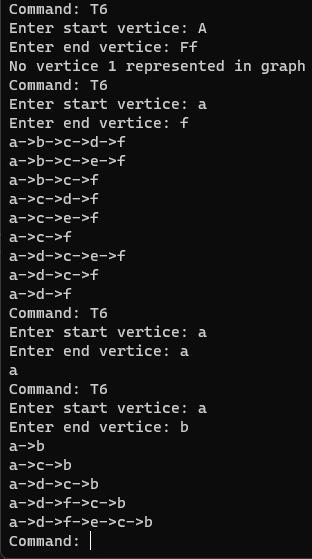
\includegraphics[scale=1]{pics/task6_1}}
	\caption{Задание 6}
	\label{pic6_1}
\end{figure}

\begin{figure}[H]
	\center{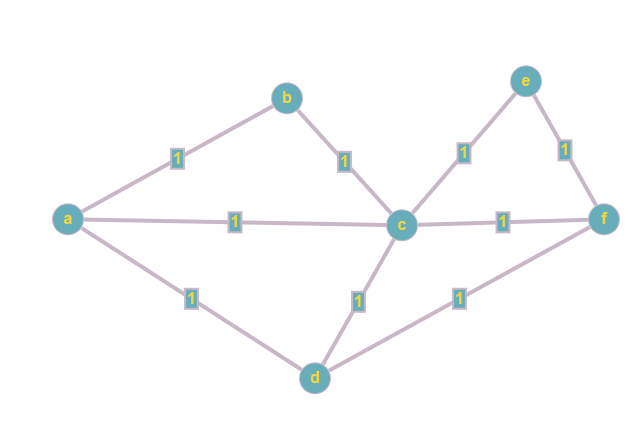
\includegraphics[scale=0.7]{pics/gr6_1}}
	\caption{Граф 6}
	\label{gr6_1}
\end{figure}

\section{Задание 7: Каркас III}

\textbf{Задание: найти во взвешенном неориентированном графе каркас минимального веса (алгоритмом Прима)}

Обычная реализация алгоритма Прима: на каждом этапе будем жадно выбирать ребро с минимальным весом, расширяющее наше дерево.

Если граф ориентированный или несвязный, то возвращаем NULL. Иначе возвращаем указатель на новосозданный каркас.

\begin{figure}[H]
	\center{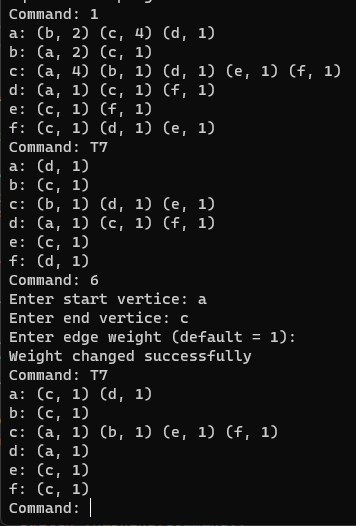
\includegraphics[scale=1]{pics/task7_1}}
	\caption{Задание 7}
	\label{pic7_1}
\end{figure}

\begin{figure}[H]
	\center{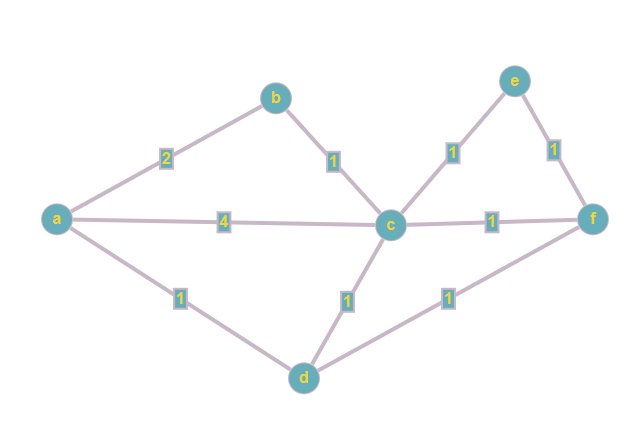
\includegraphics[scale=0.7]{pics/gr7_1}}
	\caption{Граф 7.1}
	\label{gr7_1}
\end{figure}

\begin{figure}[H]
	\center{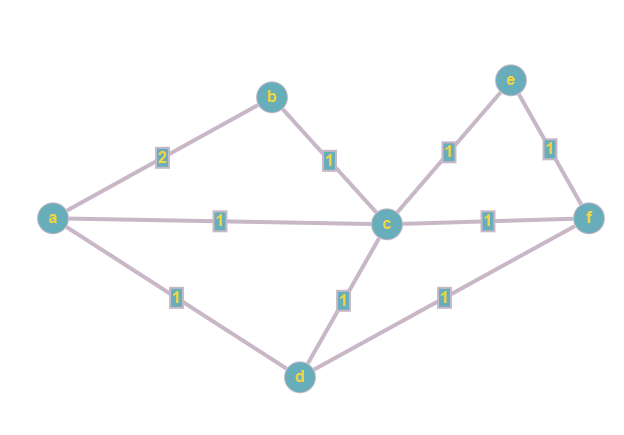
\includegraphics[scale=0.7]{pics/gr7_2}}
	\caption{Граф 7.2}
	\label{gr7_2}
\end{figure}
\section{Задание 8: Веса IVc}

\textbf{Задание: Эксцентриситет вершины — максимальное расстояние из всех минимальных расстояний от других вершин до данной вершины. Радиус графа — минимальный из эксцентриситетов его вершин. Найти центр графа — множество вершин, эксцентриситеты которых равны радиусу графа. В графе нет рёбер отрицательного веса.}

Используем обычный алгоритм Дейкстры для обхода графа и нахождения всевозможных расстояний от одной вершины до другой. Затем считаем максимум среди этих расстояний (эксцентриситеты), а затем минимумы из этих максимумов (минимум эксцентриситетов -- радиус графа). Затем соотносим найденный радиус с минимальным эксцентриситетом каждой вершины: если они совпадают, то эта вершина входит в центр графа.

Если граф несвязный, то его радиус -- $+\infty$. В таком случае его нет, сообщаем об этом. В ином случае выводим множество вершин.

\begin{figure}[H]
	\center{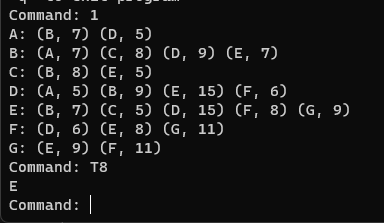
\includegraphics[scale=0.9]{pics/task8_1}}
	\caption{Задание 8}
	\label{pic8_1}
\end{figure}

\begin{figure}[H]
	\center{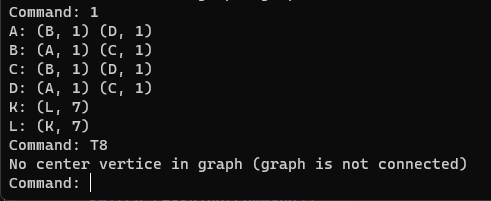
\includegraphics[scale=0.9]{pics/task8_2}}
	\caption{Задание 8}
	\label{pic8_2}
\end{figure}

\begin{figure}[H]
	\center{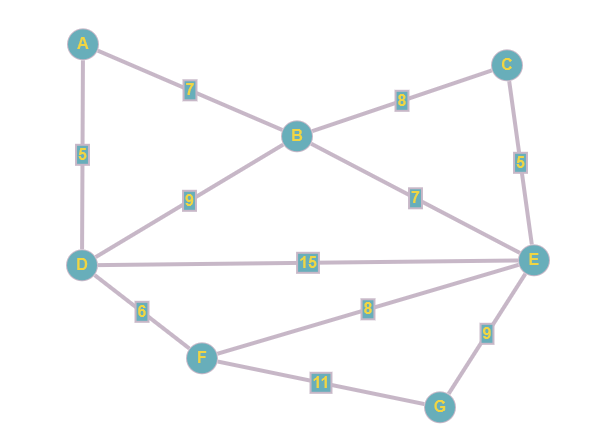
\includegraphics[scale=0.7]{pics/gr8_1}}
	\caption{Граф 8.2}
	\label{gr8_1}
\end{figure}

\begin{figure}[H]
	\center{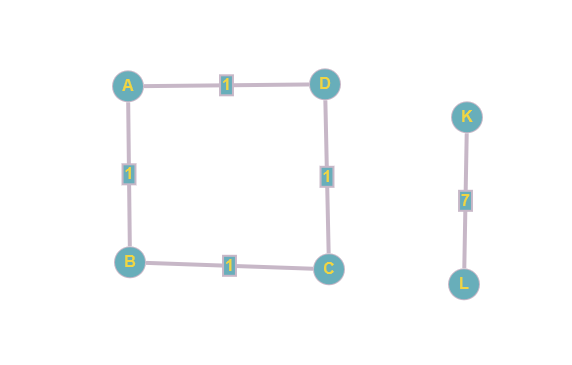
\includegraphics[scale=0.7]{pics/gr8_2}}
	\caption{Граф 8.1}
	\label{gr8_2}
\end{figure}
\section{Задание 9: Веса IVc}

\textbf{Задание: Вывести кратчайшие пути для всех пар вершин. В графе нет циклов отрицательного веса.}

Воспользуемся алгоритмом Флойда, который также запоминает путь, по которому был получен данный кратчайший путь. Затем просто выводим эти кратчайшие пути с минимальным найденным расстоянием.

Если найден отрицательный цикл, то алгоритм останавливается и выводит сообщение об ошибке.

\begin{figure}[H]
	\center{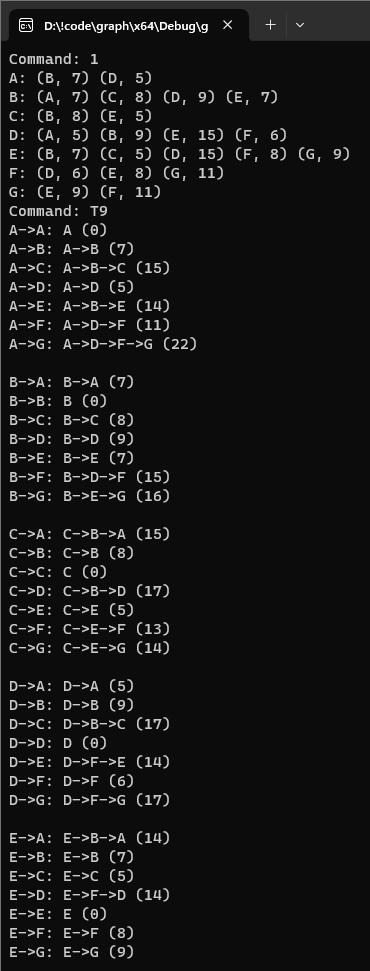
\includegraphics[scale=0.7]{pics/task9_1}}
	\caption{Задание 9}
	\label{pic9_1}
\end{figure}

\begin{figure}[H]
	\center{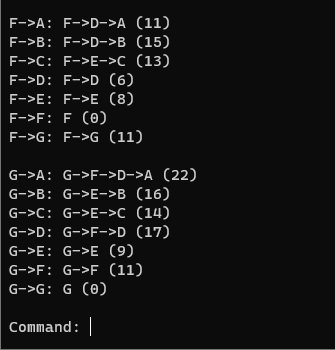
\includegraphics[scale=0.8]{pics/task9_2}}
	\caption{Задание 9}
	\label{pic9_2}
\end{figure}

\begin{figure}[H]
	\center{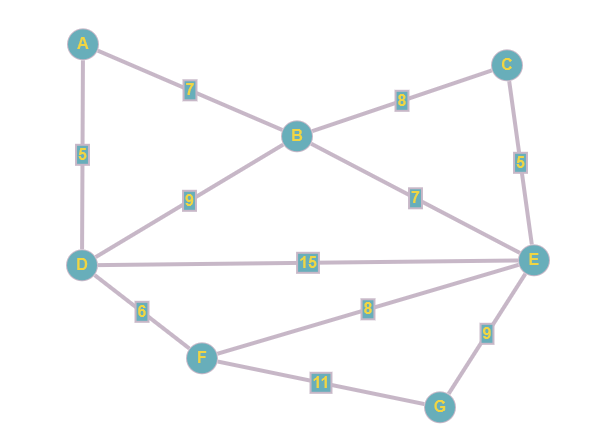
\includegraphics[scale=0.7]{pics/gr9_1}}
	\caption{Граф 9.1}
	\label{gr9_1}
\end{figure}

\begin{figure}[H]
	\center{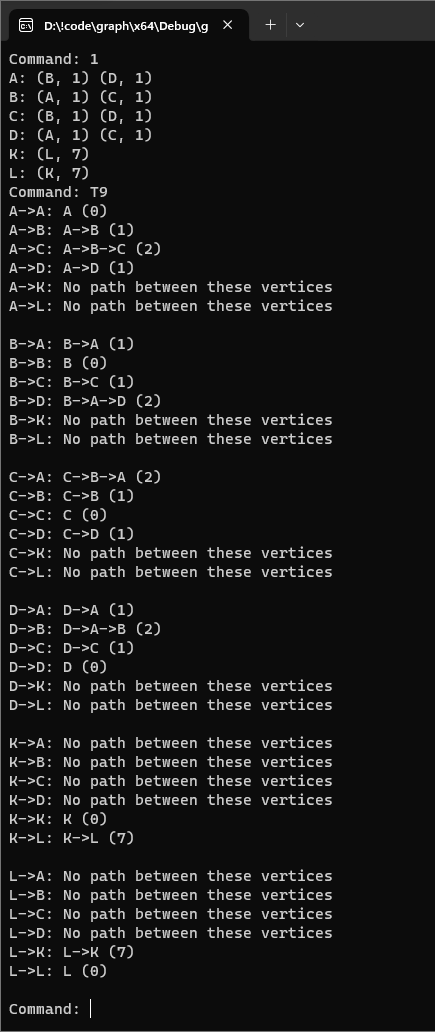
\includegraphics[scale=0.8]{pics/task9_3}}
	\caption{Задание 9}
	\label{pic9_3}
\end{figure}

\begin{figure}[H]
	\center{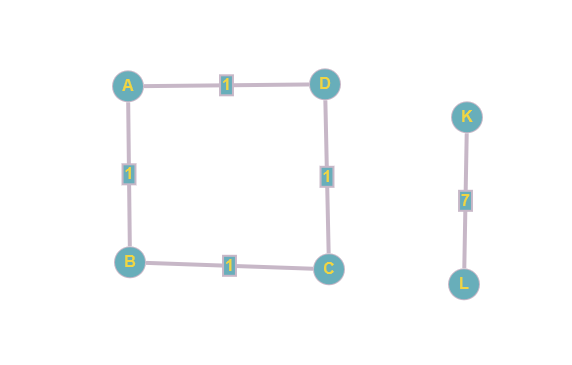
\includegraphics[scale=0.8]{pics/gr9_2}}
	\caption{Граф 9.2}
	\label{gr9_2}
\end{figure}

\begin{figure}[H]
	\center{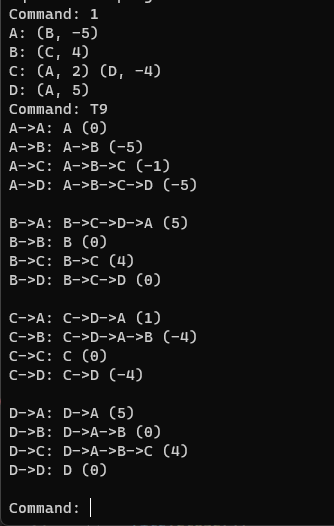
\includegraphics[scale=0.8]{pics/task9_4}}
	\caption{Задание 9}
	\label{pic9_4}
\end{figure}

\begin{figure}[H]
	\center{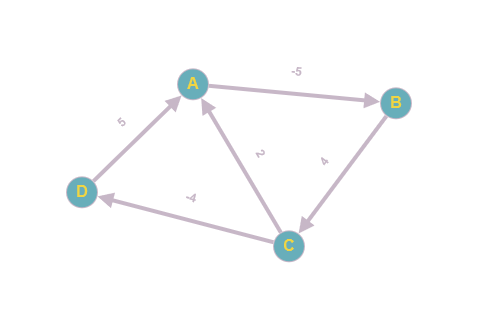
\includegraphics[scale=0.9]{pics/gr9_3}}
	\caption{Граф 9.3}
	\label{gr9_3}
\end{figure}
\section{Задание 10: Веса IVc}

\textbf{Задание: Определить, существует ли путь длиной не более L между двумя заданными вершинами графа.}

Воспользуемся алгоритмом Форда-Беллмана. При нахождении отрицательного цикла останавливаем алгоритм и выводим сообщение об ошибке. Затем соотносим кратчайший путь с величиной L: если кратчайший путь меньше, то путь существует (предъявляем его), иначе выводим сообщение о том, что он не существует.

\begin{figure}[H]
	\center{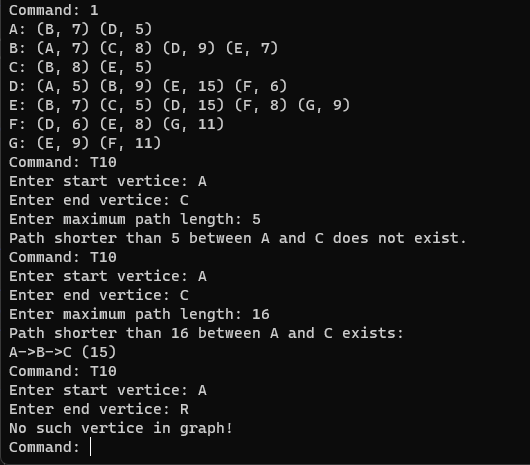
\includegraphics[scale=0.65]{pics/task10_1}}
	\caption{Задание 10}
	\label{pic10_1}
\end{figure}

\begin{figure}[H]
	\center{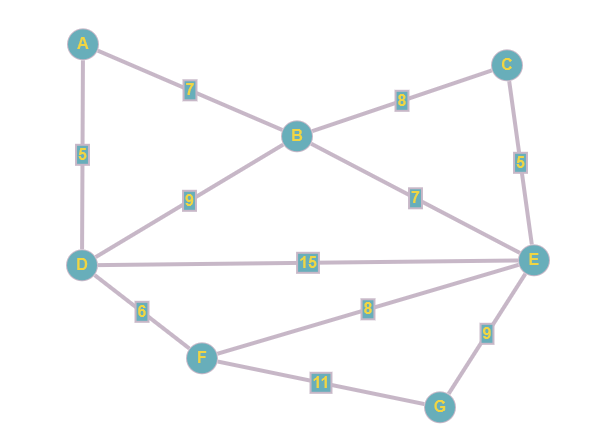
\includegraphics[scale=0.65]{pics/gr10_1}}
	\caption{Граф 10.1}
	\label{gr10_1}
\end{figure}

\begin{figure}[H]
	\center{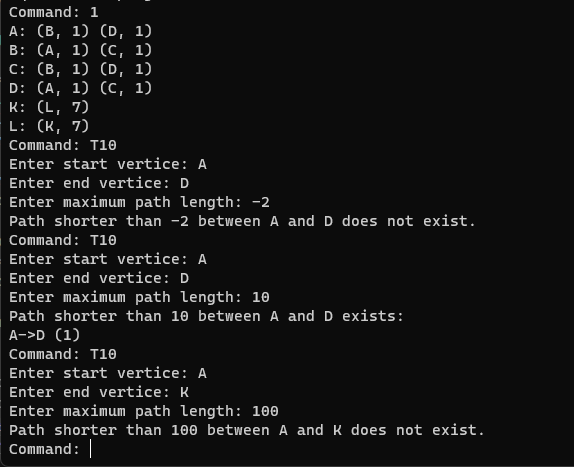
\includegraphics[scale=0.7]{pics/task10_2}}
	\caption{Задание 10}
	\label{pic10_2}
\end{figure}

\begin{figure}[H]
	\center{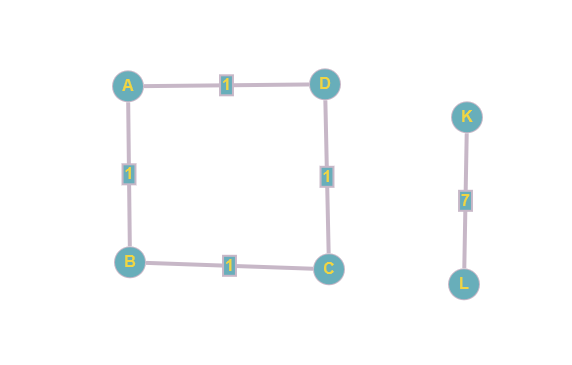
\includegraphics[scale=0.8]{pics/gr10_2}}
	\caption{Граф 10.2}
	\label{gr10_2}
\end{figure}

\begin{figure}[H]
	\center{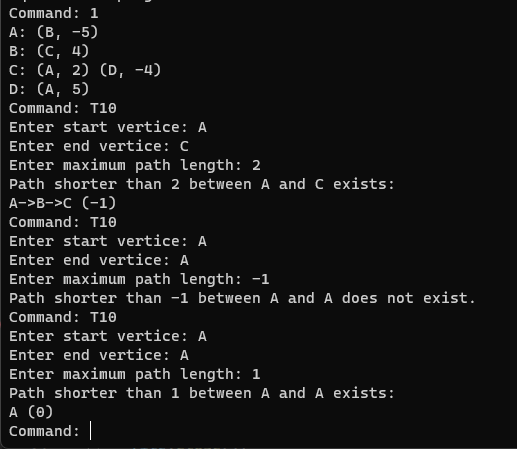
\includegraphics[scale=0.7]{pics/task10_3}}
	\caption{Задание 10}
	\label{pic10_3}
\end{figure}

\begin{figure}[H]
	\center{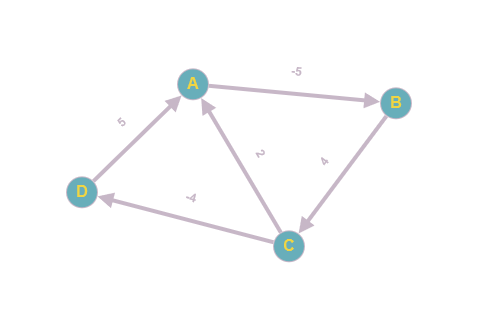
\includegraphics[scale=0.8]{pics/gr10_3}}
	\caption{Граф 10.3}
	\label{gr10_3}
\end{figure}

\begin{figure}[H]
	\center{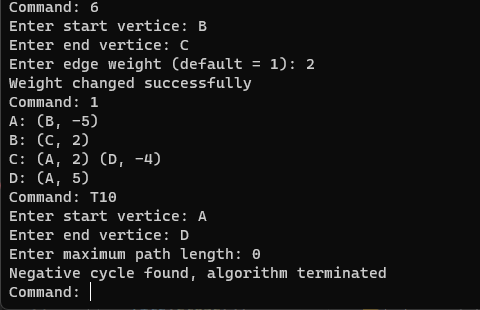
\includegraphics[scale=0.8]{pics/task10_4}}
	\caption{Задание 10}
	\label{pic10_4}
\end{figure}

\begin{figure}[H]
	\center{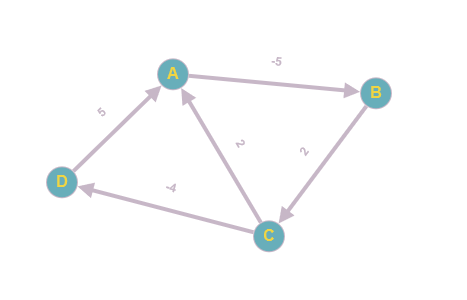
\includegraphics[scale=0.8]{pics/gr10_4}}
	\caption{Граф 10.4}
	\label{gr10_4}
\end{figure}
\section{Задание 11: Максимальный поток}

\textbf{Задание: Решить задачу на нахождение максимального потока любым алгоритмом.}

Простейшая реализация алгоритма Форда-Фалкерсона с корректировкой остаточной сети после каждого нахождения пути. Для нахождения пути используется DFS. 

\begin{figure}[H]
	\center{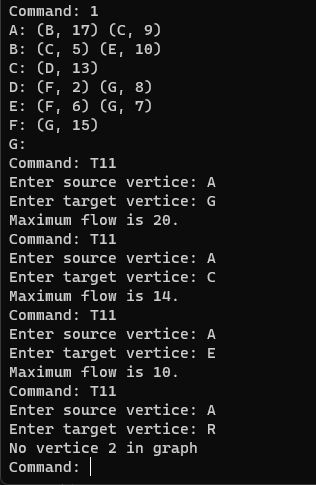
\includegraphics[scale=0.8]{pics/task11_1}}
	\caption{Задание 11}
	\label{pic11_1}
\end{figure}

\begin{figure}[H]
	\center{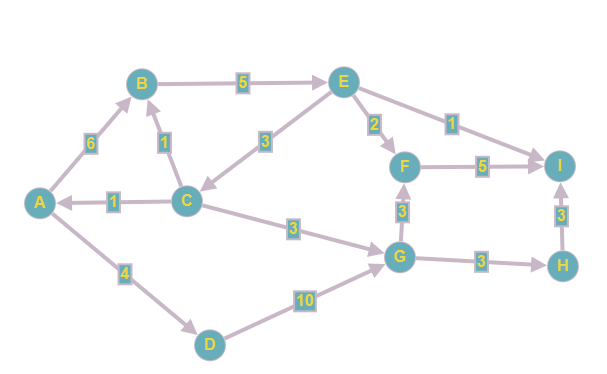
\includegraphics[scale=0.7]{pics/gr11_1}}
	\caption{Граф 11.1}
	\label{gr11_1}
\end{figure}

\begin{figure}[H]
	\center{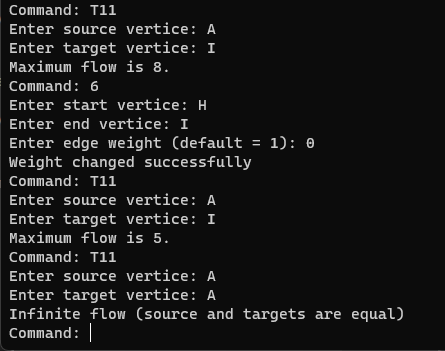
\includegraphics[scale=0.8]{pics/task11_2}}
	\caption{Задание 11}
	\label{pic11_2}
\end{figure}

\begin{figure}[H]
	\center{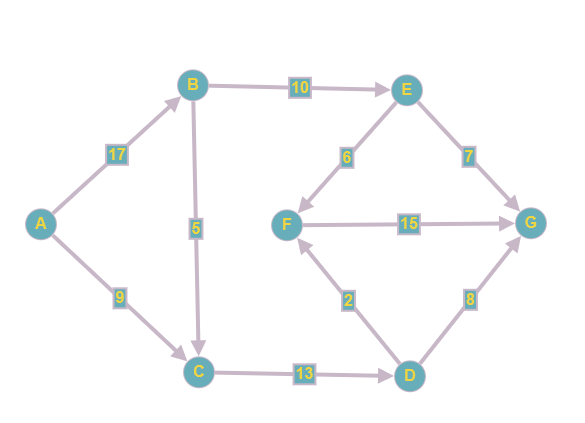
\includegraphics[scale=0.7]{pics/gr11_2}}
	\caption{Граф 11.2}
	\label{gr11_2}
\end{figure}

% Раздел "Заключение"

% \conclusion

% В этом реферате были рассмотрены основные инструменты DevOps инженера. 

% Библиографический список, составленный вручную, без использования BibTeX
%
% \begin{thebibliography}{99}
%   \bibitem{Ione} Источник 1.
%   \bibitem{Itwo} Источник 2
% \end{thebibliography}

% Отобразить все источники. Даже те, на которые нет ссылок.
\nocite{*}

% Меняем inputencoding на лету, чтобы работать с библиографией в кодировке
% `cp1251', в то время как остальной документ находится в кодировке `utf8'
\inputencoding{cp1251}
\bibliographystyle{gost780uv}
\bibliography{thesis1}
\inputencoding{utf8}

\appendix
\section{Файлы класса графов}
\label{Graph}

\textbf{Graph.h файл:}
\begin{minted}[linenos, breaklines=true, style=bw]{c++}
#pragma once

#include <map>
#include <iostream>
#include <fstream>
#include <string>
#include <nlohmann/json.hpp>

using json = nlohmann::json;

using std::string;
using std::map;
using std::vector;
using std::pair;
using std::ofstream;
using std::ifstream;

class Graph
{
	friend void to_json(json& j, const Graph& graph);
public:

	enum graph_orientation
	{
		undirected = 0,
		directed = 1
	};

	enum code_error
	{
		no_error = 0,

		vertice_exists,
		no_vertice1,
		no_vertice2,
		edge_exists,
		no_edge
	};

	Graph(bool orient = true);
	Graph(ifstream& file);
	Graph(const Graph& copiedValue);
	Graph(map<string, map<string, int32_t>>, bool isOriented);

	const map<string, map<string, int32_t>> GetAdjacencyList() const;
	bool GetOrientation();
	void ChangeOrientation();

	bool isVertice(string s);
	bool isEdge(string s1, string s2);
	
	static graph_orientation Hashing(string const& inString);

	uint8_t AddVertice(const string& value);
	uint8_t AddEdge(const string& startVertice, const string& endVertice, const int32_t& weight);

	uint8_t RemoveVertice(const string& vertice);
	uint8_t RemoveEdge(const string& startVertice, const string& endVertice);

	uint8_t ChangeWeight(const string& startVertice, const string& endVertice, const int32_t& weight);
	void Unweight();

	void Save(string fileName);
private:
	map<string, map<string, int32_t>> adjacencyList;
	bool isOriented;
};
\end{minted}

\textbf{Graph.cpp файл:}

\begin{minted}[linenos, breaklines=true, style=bw]{c++}
#include "Graph.h"

Graph::Graph(bool isOriented)
{
	this->isOriented = isOriented;
}

Graph::Graph(ifstream& file)
{
	json j;
	file >> j;
	this->isOriented = j["orient"];
	for (auto& adjList : j["vertices"].items())
	{
		this->adjacencyList[adjList.key()] = j["vertices"][adjList.key()].get<map<string, int32_t>>();
	}
}

Graph::Graph(const Graph& copiedValue)
{
	this->isOriented = copiedValue.isOriented;
	this->adjacencyList = copiedValue.adjacencyList;
}

Graph::Graph(map <string, map<string, int32_t>> list, bool isOriented)
{
	this->adjacencyList = list;
	this->isOriented = isOriented;
}

//getters
const map<string, map<string, int32_t>> Graph::GetAdjacencyList() const
{
	return adjacencyList;
}

bool Graph::GetOrientation()
{
	return isOriented;
}

void Graph::ChangeOrientation()
{
	isOriented = !isOriented;
}

bool Graph::isVertice(string s)
{
	return !(adjacencyList.find(s) == adjacencyList.end());
}

bool Graph::isEdge(string s1, string s2)
{
	return adjacencyList[s1].find(s2) != adjacencyList[s1].end();
}


Graph::graph_orientation Graph::Hashing(std::string const& inString)
{
	if (inString == "0") 
		return graph_orientation::undirected;
	else 
		return graph_orientation::directed;
}

//methods
uint8_t Graph::AddVertice(const string& vertice)
{
	if (!isVertice(vertice))
	{
		adjacencyList[vertice];
		return code_error::no_error;
	}
	else
		return code_error::vertice_exists;
}

uint8_t Graph::ChangeWeight(const string& startVertice, const string& endVertice, const int32_t& weight)
{
	//fail: no first vertice
	if (!isVertice(startVertice))
		return code_error::no_vertice1;

	//fail: no second vertice
	if (!isVertice(endVertice))
		return code_error::no_vertice2;

	//fail: no such edge
	if (!isEdge(startVertice, endVertice))
		return code_error::no_edge;

	//success
	adjacencyList[startVertice][endVertice] = weight;
	if (!isOriented)
		adjacencyList[endVertice][startVertice] = weight;
	return code_error::no_error;	
}

uint8_t Graph::AddEdge(const string& startVertice, const string& endVertice, const int32_t& weight)
{
	//fail: no first vertice
	if (!isVertice(startVertice))
		return code_error::no_vertice1;

	//fail: no second vertice
	if (!isVertice(endVertice))
		return code_error::no_vertice2;

	//fail: edge already exists
	if (isEdge(startVertice, endVertice))
		return code_error::edge_exists;

	//success
	adjacencyList[startVertice][endVertice] = weight;
	if (!isOriented)
		adjacencyList[endVertice][startVertice] = weight;
	return code_error::no_error;
}

uint8_t Graph::RemoveVertice(const string& removedVertice)
{
	//fail: no such vertice
	if (!isVertice(removedVertice))
		return code_error::no_vertice1;

	//success, cleaning other vertices and their edges
	for (auto vert : adjacencyList)
	{
		this->RemoveEdge(vert.first, removedVertice);
		this->RemoveEdge(removedVertice, vert.first);
	}
	adjacencyList.erase(removedVertice);
	return code_error::no_error;
}

uint8_t Graph::RemoveEdge(const string& startVertice, const string& endVertice)
{
	if (adjacencyList[startVertice].find(endVertice) != adjacencyList[startVertice].end())
	{
		adjacencyList[startVertice].erase(endVertice);
		if (!isOriented)
		{
			adjacencyList[endVertice].erase(startVertice);
		}
		//success
		return no_error;
	}
	else
		return code_error::no_edge;
}

void Graph::Unweight()
{
	for (auto vert1 = adjacencyList.begin(); vert1 != adjacencyList.end(); vert1++)
	{
		for (auto vert2 = adjacencyList.begin(); vert2 != adjacencyList.end(); vert2++)
		{
			if (isEdge(vert1->first, vert2->first))
				adjacencyList [vert1->first][vert2->first] = 1;
		}
	}
}

void Graph::Save(string fileName)
{
	json j = *this;
	std::ofstream data(fileName);
	data << std::setw(4) << j;
}

void to_json(json& j, const Graph& graph)
{
	j["orient"] = graph.isOriented;
	for (auto const& mapEl : graph.adjacencyList)
	{
		j["vertices"][mapEl.first] = mapEl.second;
	}
}
\end{minted}

\section{Файлы класса приложения}
\label{App}
\textbf{App.h}

\begin{minted}[linenos, breaklines=true, style=bw]{c++}
#pragma once

#include <string>
#include <iostream>

#include "Graph.h"

enum string_code
{
	printVertices = 1,
	addVertice,
	removeVertice,
	addEdge,
	removeEdge,
	changeWeight,
	saveGraph,
	unweightGraph,

	task2 = 10,
	task3,
	task4,
	task5,
	task6,
	task7,
	task8,
	task9,
	task10,
	task11,

	help = 30,
	quit
};

string_code Hashing(std::string const& inString);
void CommandMessage();
Graph* CreateGraph(string& command);

bool is_number(const string& s);
void PrintVertices(Graph* graph);
void AddVertice(Graph* graph);
void RemoveVertice(Graph* graph);
void AddEdge(Graph* graph);
void RemoveEdge(Graph* graph);
void ChangeWeight(Graph* graph);
void Unweight(Graph* graph);
\end{minted}

\textbf{App.cpp}

\begin{minted}[linenos, breaklines=true, style=bw]{c++}
#include "App.h"

using std::string;
using std::getline;
using std::cin;
using std::cout;

string_code Hashing(std::string const& inString) {
	if (inString == "1") return printVertices;
	if (inString == "2") return addVertice;
	if (inString == "3") return removeVertice;
	if (inString == "4") return addEdge;
	if (inString == "5") return removeEdge;
	if (inString == "6") return changeWeight;
	if (inString == "7") return saveGraph;
	if (inString == "8") return unweightGraph;

	if (inString == "T2") return task2;
	if (inString == "T3") return task3;
	if (inString == "T4") return task4;
	if (inString == "T5") return task5;
	if (inString == "T6") return task6;
	if (inString == "T7") return task7;
	if (inString == "T8") return task8;
	if (inString == "T9") return task9;
	if (inString == "T10") return task10;
	if (inString == "T11") return task11;

	if (inString == "h") return help;
	if (inString == "q") return quit;
}

void CommandMessage()
{
	std::cout << "Select command:\n"
		<< "1 - Print Vertices\n"
		<< "2 - Add vertice\n"
		<< "3 - Remove vertice\n"
		<< "4 - Add edge\n"
		<< "5 - Remove edge\n"
		<< "6 - Change edge's weight\n"
		<< "7 - Save graph\n"
		<< "8 - Unweight graph\n"
		<< '\n'
		<< "T2 - task 2\n"
		<< "T3 - task 3\n"
		<< "T4 - task 4\n"
		<< "T5 - task 5\n"
		<< "T6 - task 6\n"
		<< "T7 - task 7\n"
		<< "T8 - task 8\n"
		<< "T9 - task 9\n"
		<< "T10 - task 10\n"
		<< "T11 - task 11\n"
		<< '\n'
		<< "'h' to print this message\n"
		<< "'q' to exit program\n";
}

Graph* CreateGraph(string& command)
{
	while (true)
	{
		std::cout << "No graph found. Choose directed or undirected graph\n"
			<< "1 - Directed graph\n"
			<< "2 - Undirected graph\n";
		getline(std::cin, command);
		switch (Graph::Hashing(command))
		{
		case Graph::undirected:
			std::cout << "Created a new undirected graph\n";
			return new Graph(false);
		case Graph::directed:
			std::cout << "Created a new directed graph\n";
			return new Graph(true);
		default:
			break;
		}
	}
}

//Hidden
bool is_number(const std::string& s)
{
	std::string::const_iterator it = s.begin();
	while (it != s.end() && (std::isdigit(*it) || (*it) == '-')) ++it;
	return !s.empty() && it == s.end();
}

void PrintVertices(Graph* graph)
{
	auto adjacencyList = graph->GetAdjacencyList();

	for (auto& list : adjacencyList)
	{
		std::cout << list.first << ": ";
		for (auto& el : list.second)
		{
			std::cout << "(" << el.first << ", " << el.second << ") ";
		}
		std::cout << '\n';
	}
}

void AddVertice(Graph* graph)
{
	string vertice;
	std::cout << "Enter vertice to add: ";
	getline(cin, vertice);
	switch (graph->AddVertice(vertice))
	{
	case Graph::code_error::no_error:
		std::cout << "Vertice added succesfully\n";
		break;
	case Graph::code_error::vertice_exists:
		std::cout << "Vertice already exists\n";
		break;
	}	
}

void RemoveVertice(Graph* graph)
{
	string vertice;
	std::cout << "Enter vertice to remove: ";
	getline(cin, vertice);
	switch (graph->RemoveVertice(vertice))
	{
	case Graph::code_error::no_error:
		std::cout << "Vertice removed successfully\n";
		break;
	case Graph::code_error::no_vertice1:
		std::cout << "No such vertice in graph\n";
		break;
	}
}

void AddEdge(Graph* graph)
{
	string vertice1;
	string vertice2;
	string weightMsg;
	std::cout << "Enter start vertice: ";
	getline(cin, vertice1);
	std::cout << "Enter end vertice: ";
	getline(cin, vertice2);
	std::cout << "Enter edge weight (default = 1): ";
	getline(cin, weightMsg);
	if (weightMsg.empty())
		weightMsg = "1";
	while (!is_number(weightMsg))
	{
		std::cout << "Wrong weight value! Enter integer: ";
		getline(cin, weightMsg);
		if (weightMsg.empty())
			weightMsg = "1";
	}

	switch (graph->AddEdge(vertice1, vertice2, std::stoi(weightMsg)))
	{
	case Graph::no_vertice1:
		std::cout << "No vertice 1 represented in graph\n";
		break;
	case Graph::no_vertice2:
		std::cout << "No vertice 2 represented in graph\n";
		break;
	case Graph::edge_exists:
		std::cout << "Edge already exists between these 2 vertices\n";
		break;
	case Graph::no_error:
		std::cout << "Edge added successfully\n";
		break;
	}
}

void RemoveEdge(Graph* graph)
{
	string vertice1;
	string vertice2;
	std::cout << "Enter start vertice: ";
	getline(cin, vertice1);
	std::cout << "Enter end vertice: ";
	getline(cin, vertice2);

	switch (graph->RemoveEdge(vertice1, vertice2))
	{
	case Graph::code_error::no_edge:
		std::cout << "No such edge in graph\n";
		break;
	case Graph::code_error::no_error:
		std::cout << "Edge removed successfully\n";
		break;
	}
}

void ChangeWeight(Graph* graph)
{
	string vertice1;
	string vertice2;
	string weightMsg;
	std::cout << "Enter start vertice: ";
	getline(cin, vertice1);
	std::cout << "Enter end vertice: ";
	getline(cin, vertice2);
	std::cout << "Enter edge weight (default = 1): ";
	getline(cin, weightMsg);
	if (weightMsg.empty())
		weightMsg = "1";
	while (!is_number(weightMsg))
	{
		std::cout << "Wrong weight value! Enter integer: ";
		getline(cin, weightMsg);
	}

	switch (graph->ChangeWeight(vertice1, vertice2, std::stoi(weightMsg)))
	{
	case Graph::no_vertice1:
		std::cout << "No vertice 1 represented in graph\n";
		break;
	case Graph::no_vertice2:
		std::cout << "No vertice 2 represented in graph\n";
		break;
	case Graph::no_edge:
		std::cout << "No edge exists between these 2 vertices\n";
		break;
	case Graph::no_error:
		std::cout << "Weight changed successfully\n";
		break;
	}
}

void Unweight(Graph* graph)
{
	graph->Unweight();
	std::cout << "Weight of all edges changed to 1\n";
}
\end{minted}

\section{Файлы Tasks (заданий)}
\label{Tasks}

\textbf{Tasks.h}

\begin{minted}[linenos, breaklines=true, style=bw]{c++}
#pragma once

#include <iostream>
#include <string>
#include <queue>
#include <string>
#include <iostream>
#include <set>
#include <stack>
#include <algorithm>

#include "Graph.h"

void task2_14(Graph* graph);
void task3_9(Graph* graph);
void task4_10(Graph* graph1, Graph* graph2);
void task5_2(Graph* graph);
void task6_20(Graph* graph);
void task7_prim(Graph* graph);
void task8_11(Graph* graph);
void task9_17(Graph* graph);
void task10_1(Graph* graph);
void task11_net(Graph* graph);
\end{minted}

\textbf{Tasks.cpp}

\begin{minted}[linenos, breaklines=true, style=bw]{c++}
#include "Tasks.h"
#include "App.h"
#include "algos.h"

using std::string;
using std::set;
using std::getline;
using std::cin;
using std::cout;

//just prints adjacent vertices
void task2_14(Graph* graph)
{
	string vertice;
	std::cout << "Enter vertice to print: ";
	getline(cin, vertice);

	auto list = graph->GetAdjacencyList();
	auto map = list[vertice];
	if (map.empty())
	{
		std::cout << "No adjacent vertices!\n";
	}
	else
	{
		std::cout << vertice << ": ";
		for (auto& el : map)
		{
			std::cout << "(" << el.first << ", " << el.second << ") ";
		}
		std::cout << '\n';
	}
}

//oriented graphs: only vertices which are reachable from current
void task3_9(Graph* graph)
{
	string vertice;
	std::cout << "Enter vertice: ";
	getline(cin, vertice);

	auto list = graph->GetAdjacencyList();
	if (list.find(vertice) == list.end())
	{
		std::cout << "No such vertice in graph\n";
		return;
	}
	auto mapTarget = list[vertice];
	uint16_t counter = 0;
	{
		for (auto el : list)
		{
			if (el.second.size() > mapTarget.size())
			{
				std::cout << el.first << ' ';
				++counter;
			}
		}
		if (!counter)
			std::cout << "No such vertices!";
		std::cout << '\n';
	}
}

void task4_10(Graph* graph1, Graph* graph2)
{
	if (graph1->GetOrientation() != graph2->GetOrientation())
	{
		std::cout << "Graphs are incompatible\n";
		return;
	}

	auto list1 = graph1->GetAdjacencyList();
	auto list2 = graph2->GetAdjacencyList();

	map<string, map<string, int32_t>> newMap;
	for (auto it : list1)
		newMap[it.first];
	for (auto it : list2)
		newMap[it.first];

	for (auto it1 : newMap)
	{
		for (auto it2 : newMap)
		{
			auto f1 = list1[it1.first].find(it2.first);
			auto f2 = list2[it1.first].find(it2.first);

			if (f1 != list1[it1.first].end() && f2 == list2[it1.first].end())
			{
				newMap[it1.first][it2.first] = list1[it1.first][it2.first];
			}
			else if (f1 == list1[it1.first].end() && f2 != list2[it1.first].end())
			{
				newMap[it1.first][it2.first] = list2[it1.first][it2.first];
			}

		}
	}
	Graph* newGraph = new Graph(newMap, graph1->GetOrientation());
	PrintVertices(newGraph);
}

void task5_2(Graph* graph)
{
	string vertice;
	std::cout << "Enter target vertice: ";
	getline(cin, vertice);
	map<string, bool> used;
	auto list = graph->GetAdjacencyList();
	bool allFound = true;
	for (auto it : list)
	{
		used[it.first] = false;
	}
	bfs(list, vertice, used);
	for (auto it : used)
	{
		if (!used[it.first])
		{
			allFound = false;
			std::cout << it.first << ' ';
		}
			
	}
	if (allFound)
		std::cout << "All vertices are reachable from " << vertice << '!';
	std::cout << '\n';
}


void task6_20(Graph* graph)
{
	string startVertice;
	string endVertice;
	auto list = graph->GetAdjacencyList();
	std::cout << "Enter start vertice: ";
	getline(cin, startVertice);
	std::cout << "Enter end vertice: ";
	getline(cin, endVertice);
	if (list.find(startVertice) == list.end())
	{
		std::cout << "No vertice 1 represented in graph\n";
		return;
	}
	if (list.find(endVertice) == list.end())
	{
		std::cout << "No vertice 2 represented in graph\n";
		return;
	}
	map<string, bool> used;
	vector<string> path;
	int32_t ans = 0;

	for (auto it : list)
	{
		used[it.first] = false;
	}
	dfs_modified(list, startVertice, endVertice, used, path, ans);
	if (!ans)
		std::cout << "No paths between these 2 vertices!\n";
}

//Prim algorithm realisation
void task7_prim(Graph* graph)
{
	Graph* tree = prim(graph);
	if (tree == nullptr)
		std::cout << "No spanning tree exists (graph should be connected and undirected)\n";
	else
		PrintVertices(tree);
}

void task8_11(Graph* graph)
{
	map<string, map<string, int32_t>> minimalDistance;
	auto list = graph->GetAdjacencyList();
	for (auto vert : list)
	{
		minimalDistance[vert.first] = dijkstra(graph, vert.first);
	}
	map<string, int32_t> eccentricity;
	int32_t radius = INT32_MAX;
	for (auto vert : minimalDistance)
	{
		eccentricity[vert.first] = std::max_element(vert.second.begin(), vert.second.end(), 
			[&](const auto p1, const auto p2) {return p1.second < p2.second; })->second;
		radius = std::min(eccentricity[vert.first], radius);
	}
	
	if (radius == INT32_MAX)
	{
		std::cout << "No center vertice in graph (graph is not connected)\n";
		return;
	}

	for (auto vert : eccentricity)
	{
		if (vert.second == radius)
			std::cout << vert.first << ' ';
	}
	cout << '\n';
	return;
}

void task9_17(Graph* graph)
{
	auto floydRes = floyd(graph);
	map<string, map<string, int32_t>> minimalDistance = floydRes.first;
	map<string, map<string, string>> pathVertices = floydRes.second;

	for (auto vert : minimalDistance)
	{
		if (vert.second[vert.first] < 0)
		{
			cout << "Negative cycle found, algorithm terminated\n";
			return;
		}
	}

	auto list = graph->GetAdjacencyList();
	std::stack<string> path;
	for (auto vert1 : list)
	{
		for (auto vert2 : list)
		{
			cout << vert1.first << "->" << vert2.first << ": ";
			if (minimalDistance[vert1.first][vert2.first] == INT32_MAX)
			{
				cout << "No path between these vertices\n";
			}
			else
			{
				WayBack(vert1.first, vert2.first, path, pathVertices);
				cout << path.top();
				path.pop();
				while (!path.empty())
				{
					cout << "->" << path.top();
					path.pop();
				}
				cout << " (" << minimalDistance[vert1.first][vert2.first] << ")" << '\n';
			}
		}
		cout << '\n';
	}
}

void task10_1(Graph* graph)
{
	//ADD VERTICE CHECKING
	string vertice1;
	string vertice2;
	string L;
	std::cout << "Enter start vertice: ";
	getline(cin, vertice1);
	if (!graph->isVertice(vertice1))
	{
		cout << "No such vertice in graph!\n";
		return;
	}
	std::cout << "Enter end vertice: ";
	getline(cin, vertice2);
	if (!graph->isVertice(vertice2))
	{
		cout << "No such vertice in graph!\n";
		return;
	}
	std::cout << "Enter maximum path length: ";
	getline(cin, L);
	if (!is_number(L))
	{
		cout << "Wrong weight value! Enter integer: ";
		return;
	}

	auto list = graph->GetAdjacencyList();
	map<string, map<string, int32_t>> minimalDistance;
	map<string, map<string, string>> pathVertices;
	for (auto vert : list)
	{
		auto algRes = ford_bellman(graph, vert.first);
		if (std::get<0>(algRes) == true)
		{
			cout << "Negative cycle found, algorithm terminated\n";
			return;
		}
		else
		{
			minimalDistance[vert.first] = std::get<1>(algRes);
			if (vert.first == vertice1)
				pathVertices[vert.first] = std::get<2>(algRes);
		}
	}
	
	if (minimalDistance[vertice1][vertice2] < std::stoi(L))
	{
		cout << "Path shorter than " << L << " between " << vertice1 << " and " << vertice2
			<< " exists:\n";
		std::stack<string> path;
		WayBack(vertice1, vertice2, path, pathVertices);
		cout << path.top();
		path.pop();
		while (!path.empty())
		{
			cout << "->" << path.top();
			path.pop();
		}
		cout << " (" << minimalDistance[vertice1][vertice2] << ")" << '\n';
	}
	else
	{
		cout << "Path shorter than " << L << " between " << vertice1 << " and " << vertice2
			<< " does not exist.\n";
	}
}

void task11_net(Graph* graph)
{
	string vertice1;
	string vertice2;
	std::cout << "Enter source vertice: ";
	getline(cin, vertice1);
	std::cout << "Enter target vertice: ";
	getline(cin, vertice2);
	if (vertice1 == vertice2)
	{
		cout << "Infinite flow (source and targets are equal)\n";
		return;
	}
	if (!graph->isVertice(vertice1))
	{
		cout << "No vertice 1 in graph\n";
		return;
	}
	if (!graph->isVertice(vertice2))
	{
		cout << "No vertice 2 in graph\n";
		return;
	}
	cout << "Maximum flow is " << ford_fulkerson(graph, vertice1, vertice2) << ".\n";
}
\end{minted}

\section{Файлы алгоритмов}
\label{Algos}

\textbf{Algos.h}

\begin{minted}[linenos, breaklines=true, style=bw]{c++}
#pragma once

#include <iostream>
#include <string>
#include <queue>
#include <iostream>
#include <map>
#include <stack>

#include "Graph.h"

void dfs_modified(
	map<string, map<string, int32_t>>& list,
	const string& current,
	const string& end,
	map<string, bool>& used,
	vector<string>& path,
	int32_t& counter);
void dfs(map<string, map<string, int32_t>>& list, const string& vertice, map<string, bool>& used);
void bfs(map<string, map<string, int32_t>>& list, const string& vertice, map<string, bool>& used);
Graph* prim(Graph* graph, string root = "");

void WayBack(const string& startSource, const string& targetSource, std::stack<string>& path,
	map<string, map<string, string>>& pathVertices);

map<string, int32_t> dijkstra(Graph* graph, string root);
pair<map<string, map<string, int32_t>>,
	map<string, map<string, string>>> floyd(Graph* graph);

std::tuple<bool, map<string, int32_t>, map<string, string>> ford_bellman(Graph* graph, string root);

int ford_fulkerson(Graph* graph, string source, string target);
\end{minted}

\textbf{Algos.cpp}
\begin{minted}[linenos, breaklines=true, style=bw]{c++}
#include "algos.h"

void dfs_modified(
	map<string, map<string, int32_t>>& list,
	const string& current,
	const string& end,
	map<string, bool>& used,
	vector<string>& path,
	int32_t& counter)
{
	if (current == end)
	{
		for (auto it = path.begin(); it != path.end(); it++)
		{
			std::cout << *it << "->";
		}
		++counter;
		std::cout << end << '\n';
		return;
	}

	used[current] = true;
	for (auto it : list[current])
	{
		if (!used[it.first])
		{
			path.push_back(current);
			dfs_modified(list, it.first, end, used, path, counter);
			path.pop_back();
		}
	}
	used[current] = false;
}

void dfs(map<string, map<string, int32_t>>& list, const string& vertice, map<string, bool>& used)
{
	used[vertice] = true;
	for (auto it : list[vertice])
	{
		if (!used[it.first])
		{
			dfs(list, it.first, used);
		}
	}
}

void bfs(map<string, map<string, int32_t>>& list, const string& vertice, map<string, bool>& used)
{
	string cur;
	std::queue<string> q;
	used[vertice] = true;
	q.push(vertice);
	while (!q.empty())
	{
		cur = q.front();
		q.pop();
		for (auto it : list[cur])
		{
			if (!used[it.first])
			{
				used[it.first] = true;
				q.push(it.first);
			}
		}
	}
}

Graph* prim(Graph* graph, string root)
{
	Graph* tree = new Graph(graph->GetOrientation());
	if (graph->GetOrientation() == true)
		return nullptr;
	auto list = graph->GetAdjacencyList();

	map<string, bool> used;
	map<string, int32_t> minEdge;
	map<string, string> prevEdge;
	for (auto it : list)
	{
		used[it.first] = false;
		minEdge[it.first] = INT32_MAX;
		prevEdge[it.first] = "";
	}

	dfs(list, list.begin()->first, used);
	for (auto it : used)
	{
		if (used[it.first] == false)
			return nullptr;
		used[it.first] = false;
	}

	if (root == "")
	{
		minEdge[list.begin()->first] = 0;
		tree->AddVertice(list.begin()->first);
	}
	else
	{
		minEdge[root] = 0;
		tree->AddVertice(root);
	}

	

	for (auto it : list)
	{
		string v = "";
		for (auto minVert : list)
		{
			if (!used[minVert.first] && (v == "" || minEdge[minVert.first] < minEdge[v]))
				v = minVert.first;
		}
		if (v == "")
		{
			//no MST
			std::cout << "No MST\n";
			return new Graph();
		}

		used[v] = true;
		if (prevEdge[v] != "")
		{
			auto treeList = tree->GetAdjacencyList();
			tree->AddVertice(v);
			tree->AddEdge(v, prevEdge[v], list[v][prevEdge[v]]);
			//std::cout << v << ' ' << prevEdge[v] << '\n';
		}

		for (auto vert : list[v])
			if (vert.second < minEdge[vert.first])
			{
				minEdge[vert.first] = vert.second;
				prevEdge[vert.first] = v;
			}
	}
	return tree;
}

map<string, int32_t> dijkstra(Graph* graph, string root)
{
	auto list = graph->GetAdjacencyList();
	map<string, int32_t> minimalDistance;
	//map<string, string> pathVertices;
	map <string, bool> used;
	for (auto vert1 : list)
	{
		minimalDistance[vert1.first] = INT32_MAX;
		//pathVertices[vert1.first] = "";
		used[vert1.first] = false;
	}
	minimalDistance[root] = 0;
	int32_t newDistance;
	string currentClosest;

	for (auto clos : list)
	{
		currentClosest = "";
		for (auto vert : minimalDistance)
		{
			if (!used[vert.first] &&
				(currentClosest == "" || minimalDistance[vert.first] < minimalDistance[currentClosest]))
			{
				currentClosest = vert.first;
			}
		}
		if (minimalDistance[currentClosest] == INT32_MAX)
			break;
		used[currentClosest] = true;
		for (auto vert : list[currentClosest])
		{
			newDistance = minimalDistance[currentClosest] + vert.second;
			if (newDistance < minimalDistance[vert.first])
			{
				minimalDistance[vert.first] = newDistance;
				//pathVertices[vert.first] = currentClosest;
			}
		}
	}
	return minimalDistance;
}

pair<map<string, map<string, int32_t>>,
	map<string, map<string, string>>> floyd(Graph* graph)
{
	auto list = graph->GetAdjacencyList();
	map<string, map<string, int32_t>> minimalDistance;
	map<string, map<string, string>> pathVertices;
	for (auto vert1 : list)
	{
		minimalDistance[vert1.first];
		pathVertices[vert1.first];
		for (auto vert2 : list)
		{
			if (vert1.second.find(vert2.first) != vert1.second.end())
			{
				minimalDistance[vert1.first][vert2.first] = vert1.second[vert2.first];
				pathVertices[vert1.first][vert2.first] = vert1.first;
			}
			else
			{
				minimalDistance[vert1.first][vert2.first] = vert1.first == vert2.first ? 0 : INT32_MAX;
				pathVertices[vert1.first][vert2.first] = "";
			}	
		}
	}

	int32_t newDistance;
	int32_t edge1, edge2;
	for (auto relaxVertice : list)
	{
		for (auto vert1 : list)
		{
			for (auto vert2 : list)
			{
				edge1 = minimalDistance[vert1.first][relaxVertice.first];
				edge2 = minimalDistance[relaxVertice.first][vert2.first]; 
				if (edge1 != INT32_MAX && edge2 != INT32_MAX)
				{
					newDistance = edge1 + edge2;
					if (newDistance < minimalDistance[vert1.first][vert2.first])
					{
						minimalDistance[vert1.first][vert2.first] = newDistance;
						pathVertices[vert1.first][vert2.first] = pathVertices[relaxVertice.first][vert2.first];
					}
				}
			}
		}
	}
	return std::make_pair(minimalDistance, pathVertices);
}

void WayBack(const string& startSource, const string& targetSource, std::stack<string>& path,
	map<string, map<string, string>>& pathVertices)
{
	path.push(targetSource);
	if (targetSource == startSource)
		return;
	WayBack(startSource, pathVertices[startSource][targetSource], path, 
		pathVertices);
}

std::tuple<bool, map<string, int32_t>, map<string, string>> ford_bellman(Graph* graph, string root)
{
	auto list = graph->GetAdjacencyList();
	map<string, int32_t> minimalDistance;
	map<string, string> pathVertices;

	for (auto vert1 : list)
	{
		pathVertices[vert1.first] = "";
		minimalDistance[vert1.first] = vert1.first == root ? 0 : INT32_MAX;
	}

	int32_t newDistance;
	for (int k = 1; k < list.size() + 1; k++)
	{
		for (auto u : list)
		{
			for (auto v : list[u.first])
			{
				if (minimalDistance[u.first] == INT32_MAX)
					continue;
				newDistance = minimalDistance[u.first] + list[u.first][v.first];
				if (newDistance < minimalDistance[v.first])
				{
					if (k == list.size())
					{
						return std::make_tuple(true, minimalDistance, pathVertices);
					}
					minimalDistance[v.first] = newDistance;
					pathVertices[v.first] = u.first;	
				}
			}
		}
	}
	return std::make_tuple(false, minimalDistance, pathVertices);
}

int dfs_network(const string& cur, const string& target, const int& minDelta, 
	map<string, map<string, int32_t>>& list,
	map<string, map<string, int32_t>>& flow,
	map<string, bool>& used)
{
	if (cur == target)
		return minDelta;
	if (used[cur] == true)
		return 0;
	used[cur] = true;
	int minDeltaNew;
	int curDelta;
	for (auto vert : list[cur])
	{
		curDelta = list[cur][vert.first] - flow[cur][vert.first];
		if (curDelta > 0)
		{
			minDeltaNew = dfs_network(vert.first, target, std::min(minDelta, curDelta), list, flow, used);
			if (minDeltaNew > 0)
			{
				flow[cur][vert.first] += minDeltaNew;
				flow[vert.first][cur] -= minDeltaNew;
				return minDeltaNew;
			}
		}
	}
	return 0;
}

//Вес ребра - это его пропускная способность
//Создаём новый map - это будет текущим потоком
int ford_fulkerson(Graph* graph, string source, string target)
{
	auto list = graph->GetAdjacencyList();
	map<string, map<string, int32_t>> flow;
	map<string, bool> used;

	for (auto vert1 : list)
	{
		used[vert1.first] = false;
		for (auto vert2 : list[vert1.first])
			flow[vert1.first][vert2.first] = 0;
	}
	
	int delta;
	int ans = 0;
	while (true)
	{
		for (auto vert1 : list)
			used[vert1.first] = false;
		delta = dfs_network(source, target, INT32_MAX, list, flow, used);
		if (delta > 0)
			ans += delta;
		else
			break;
	}

	return ans;
}
\end{minted}

\section{Файл Main.cpp}
\label{Main}

\textbf{main.cpp}

\begin{minted}[linenos, breaklines=true, style=bw]{c++}
#include <iostream>
#include <fstream>
#include <string>
#include <map>

#include "Graph.h"
#include "App.h"
#include "Tasks.h"

const string DATA_FILE1 = "task11_2.json";
const string DATA_FILE2 = "data4.json";

int main()
{
	string command;

	Graph* graph1;
	std::ifstream file(DATA_FILE1);
	if (file.is_open())
		graph1 = new Graph(file);
	else
		graph1 = CreateGraph(command);
	file.close();

	file.open(DATA_FILE2);
	Graph* graph2 = new Graph(file);
	file.close();

	CommandMessage();
	while (true)
	{
		std::cout << "Command: ";
		std::getline(std::cin, command);
		switch (Hashing(command))
		{
		case string_code::printVertices:
			PrintVertices(graph1);
			break;
		case string_code::addVertice:
			AddVertice(graph1);
			break;
		case string_code::removeVertice:
			RemoveVertice(graph1);
			break;
		case string_code::addEdge:
			AddEdge(graph1);
			break;
		case string_code::removeEdge:
			RemoveEdge(graph1);
			break;
		case string_code::changeWeight:
			ChangeWeight(graph1);
			break;
		case string_code::unweightGraph:
			Unweight(graph1);
			break;

		case string_code::saveGraph:
			graph1->Save(DATA_FILE1);
			std::cout << "Graph saved succesfully\n";
			break;

		case string_code::task2:
			task2_14(graph1);
			break;
		case string_code::task3:
			task3_9(graph1);
			break;
		case string_code::task4:
			task4_10(graph1, graph2);
			break;
		case string_code::task5:
			task5_2(graph1);
			break;
		case string_code::task6:
			task6_20(graph1);
			break;
		case string_code::task7:
			task7_prim(graph1);
			break;
		case string_code::task8:
			task8_11(graph1);
			break;
		case string_code::task9:
			task9_17(graph1);
			break;
		case string_code::task10:
			task10_1(graph1);
			break;
		case string_code::task11:
			task11_net(graph1);
			break;

		case string_code::help:
			CommandMessage();
			break;
		case string_code::quit:
			graph1->Save(DATA_FILE1);
			return 0;

		default:
			std::cout << "Wrong Command Number\n";
		}		
	}
}
\end{minted}

\section{Используемые для тестирования файлы}
\label{Json-файлы}

\texttt{task1\_1.json}
\begin{minted}[linenos, breaklines=true, style=bw]{js}
{
    "orient": false,
    "vertices": {
        "A": {
            "B": 1,
            "C": 1
        },
        "B": {
            "A": 1,
            "C": 1
        },
        "C": {
            "A": 1,
            "B": 1
        }
    }
}
\end{minted}
\texttt{task2\_1.json}
\begin{minted}[linenos, breaklines=true, style=bw]{js}
{
    "orient": true,
    "vertices": {
        "a": {
            "e": 1,
            "m": 1
        },
        "b": {
            "c": 1
        },
        "c": {
            "b": 9,
            "c": 3
        },
        "d": {
            "k": 1
        },
        "e": {
            "a": 1,
            "d": 1,
            "k": 1
        },
        "g": {},
        "k": {},
        "l": {
            "a": 1
        },
        "m": {
            "n": 6
        },
        "n": {}
    }
}
\end{minted}
\texttt{task3\_1.json}
\begin{minted}[linenos, breaklines=true, style=bw]{js}
{
    "orient": true,
    "vertices": {
        "a": {
            "e": 3
        },
        "b": {
            "a": 1
        },
        "c": {},
        "d": {
            "k": 1
        },
        "e": {
            "l": 9
        },
        "k": {},
        "l": {
            "k": 1
        },
        "u": {
            "v": 5
        },
        "v": {
            "a": 150,
            "c": 3
        }
    }
}
\end{minted}
\texttt{task4\_1.json}
\begin{minted}[linenos, breaklines=true, style=bw]{js}
{
    "orient": true,
    "vertices": {
        "a": {
            "b": 1
        },
        "b": {
            "a": 1,
            "c": 1
        },
        "c": {
            "b": 1
        },
        "d": {
            "e": 1
        },
        "e": {
            "d": 1,
            "f": 5
        },
        "f": {
            "e": -3,
            "n": 14
        },
        "n": {},
        "o": {}
    }
}
\end{minted}
\texttt{task4\_2.json}
\begin{minted}[linenos, breaklines=true, style=bw]{js}
{
    "orient": true,
    "vertices": {
        "a": {
            "e": 1,
            "m": 1
        },
        "b": {
            "c": 1
        },
        "c": {
            "b": 9,
            "c": 3
        },
        "d": {
            "e": 7,
            "k": 1
        },
        "e": {
            "a": 1,
            "d": 1,
            "k": 1
        },
        "g": {
            "k": 33
        },
        "k": {},
        "l": {
            "a": 1
        },
        "m": {}
    }
}
\end{minted}
\texttt{task5\_1.json}
\begin{minted}[linenos, breaklines=true, style=bw]{js}
{
    "orient": true,
    "vertices": {
        "A": {
            "B": 1
        },
        "B": {
            "D": 1
        },
        "C": {
            "B": 1,
            "D": 1,
            "E": 1
        },
        "D": {
            "G": 1,
            "L": 1
        },
        "E": {
            "C": 1,
            "F": 1,
            "G": 1
        },
        "F": {
            "A": 1
        },
        "G": {
            "A": 1
        },
        "K": {
            "L": 1
        },
        "L": {}
    }
}
\end{minted}
\texttt{task6\_1.json}
\begin{minted}[linenos, breaklines=true, style=bw]{js}
{
    "orient": false,
    "vertices": {
        "a": {
            "b": 1,
            "c": 1,
            "d": 1
        },
        "b": {
            "a": 1,
            "c": 1
        },
        "c": {
            "a": 1,
            "b": 1,
            "d": 1,
            "e": 1,
            "f": 1
        },
        "d": {
            "a": 1,
            "c": 1,
            "f": 1
        },
        "e": {
            "c": 1,
            "f": 1
        },
        "f": {
            "c": 1,
            "d": 1,
            "e": 1
        }
    }
}
\end{minted}
\texttt{task7\_1.json}
\begin{minted}[linenos, breaklines=true, style=bw]{js}
{
    "orient": false,
    "vertices": {
        "a": {
            "b": 2,
            "c": 1,
            "d": 1
        },
        "b": {
            "a": 2,
            "c": 1
        },
        "c": {
            "a": 1,
            "b": 1,
            "d": 1,
            "e": 1,
            "f": 1
        },
        "d": {
            "a": 1,
            "c": 1,
            "f": 1
        },
        "e": {
            "c": 1,
            "f": 1
        },
        "f": {
            "c": 1,
            "d": 1,
            "e": 1
        }
    }
}
\end{minted}
\texttt{task8\_1.json}
\begin{minted}[linenos, breaklines=true, style=bw]{js}
{
    "orient": false,
    "vertices": {
        "A": {
            "B": 7,
            "D": 5
        },
        "B": {
            "A": 7,
            "C": 8,
            "D": 9,
            "E": 7
        },
        "C": {
            "B": 8,
            "E": 5
        },
        "D": {
            "A": 5,
            "B": 9,
            "E": 15,
            "F": 6
        },
        "E": {
            "B": 7,
            "C": 5,
            "D": 15,
            "F": 8,
            "G": 9
        },
        "F": {
            "D": 6,
            "E": 8,
            "G": 11
        },
        "G": {
            "E": 9,
            "F": 11
        }
    }
}
\end{minted}
\texttt{task8\_2.json}
\begin{minted}[linenos, breaklines=true, style=bw]{js}
{
    "orient": false,
    "vertices": {
        "A": {
            "B": 1,
            "D": 1
        },
        "B": {
            "A": 1,
            "C": 1
        },
        "C": {
            "B": 1,
            "D": 1
        },
        "D": {
            "A": 1,
            "C": 1
        },
        "K": {
            "L": 7
        },
        "L": {
            "K": 7
        }
    }
}
\end{minted}
\texttt{task9\_1.json}
\begin{minted}[linenos, breaklines=true, style=bw]{js}
{
    "orient": false,
    "vertices": {
        "A": {
            "B": 7,
            "D": 5
        },
        "B": {
            "A": 7,
            "C": 8,
            "D": 9,
            "E": 7
        },
        "C": {
            "B": 8,
            "E": 5
        },
        "D": {
            "A": 5,
            "B": 9,
            "E": 15,
            "F": 6
        },
        "E": {
            "B": 7,
            "C": 5,
            "D": 15,
            "F": 8,
            "G": 9
        },
        "F": {
            "D": 6,
            "E": 8,
            "G": 11
        },
        "G": {
            "E": 9,
            "F": 11
        }
    }
}
\end{minted}
\texttt{task9\_2.json}
\begin{minted}[linenos, breaklines=true, style=bw]{js}
{
    "orient": false,
    "vertices": {
        "A": {
            "B": 1,
            "D": 1
        },
        "B": {
            "A": 1,
            "C": 1
        },
        "C": {
            "B": 1,
            "D": 1
        },
        "D": {
            "A": 1,
            "C": 1
        },
        "K": {
            "L": 7
        },
        "L": {
            "K": 7
        }
    }
}
\end{minted}
\texttt{task9\_3.json}
\begin{minted}[linenos, breaklines=true, style=bw]{js}
{
    "orient": true,
    "vertices": {
        "A": {
            "B": -5
        },
        "B": {
            "C": 4
        },
        "C": {
            "A": 2,
            "D": -4
        },
        "D": {
            "A": 5
        }
    }
}
\end{minted}
\texttt{task10\_1.json}
\begin{minted}[linenos, breaklines=true, style=bw]{js}
{
    "orient": false,
    "vertices": {
        "A": {
            "B": 7,
            "D": 5
        },
        "B": {
            "A": 7,
            "C": 8,
            "D": 9,
            "E": 7
        },
        "C": {
            "B": 8,
            "E": 5
        },
        "D": {
            "A": 5,
            "B": 9,
            "E": 15,
            "F": 6
        },
        "E": {
            "B": 7,
            "C": 5,
            "D": 15,
            "F": 8,
            "G": 9
        },
        "F": {
            "D": 6,
            "E": 8,
            "G": 11
        },
        "G": {
            "E": 9,
            "F": 11
        }
    }
}
\end{minted}
\texttt{task10\_2.json}
\begin{minted}[linenos, breaklines=true, style=bw]{js}
{
    "orient": false,
    "vertices": {
        "A": {
            "B": 1,
            "D": 1
        },
        "B": {
            "A": 1,
            "C": 1
        },
        "C": {
            "B": 1,
            "D": 1
        },
        "D": {
            "A": 1,
            "C": 1
        },
        "K": {
            "L": 7
        },
        "L": {
            "K": 7
        }
    }
}
\end{minted}
\texttt{task10\_3.json}
\begin{minted}[linenos, breaklines=true, style=bw]{js}
{
    "orient": true,
    "vertices": {
        "A": {
            "B": -5
        },
        "B": {
            "C": 2
        },
        "C": {
            "A": 2,
            "D": -4
        },
        "D": {
            "A": 5
        }
    }
}
\end{minted}
\texttt{task11\_1.json}
\begin{minted}[linenos, breaklines=true, style=bw]{js}
{
    "orient": true,
    "vertices": {
        "A": {
            "B": 17,
            "C": 9
        },
        "B": {
            "C": 5,
            "E": 10
        },
        "C": {
            "D": 13
        },
        "D": {
            "F": 2,
            "G": 8
        },
        "E": {
            "F": 6,
            "G": 7
        },
        "F": {
            "G": 15
        },
        "G": {}
    }
}
\end{minted}
\texttt{task11\_2.json}
\begin{minted}[linenos, breaklines=true, style=bw]{js}
{
    "orient": true,
    "vertices": {
        "A": {
            "B": 6,
            "D": 4
        },
        "B": {
            "E": 5
        },
        "C": {
            "A": 1,
            "B": 1,
            "G": 3
        },
        "D": {
            "G": 10
        },
        "E": {
            "C": 3,
            "F": 2,
            "I": 1
        },
        "F": {
            "I": 5
        },
        "G": {
            "F": 3,
            "H": 3
        },
        "H": {
            "I": 0
        },
        "I": {}
    }
}
\end{minted}

% При использовании biblatex вместо bibtex
%\printbibliography

% Окончание основного документа и начало приложений Каждая последующая секция
% документа будет являться приложением
\end{document}
